% !TEX root = main.tex
% 有阻尼的受迫振子

\section{有阻尼的受迫振子}%
油,蜂蜜等浓的液体中,摩擦和速度成正比
\begin{equation*}
	f \propto v
\end{equation*}

\begin{equation*}
	f = -m \gamma \dot{x}
\end{equation*}

\begin{equation*}
	m \ddot{x} = F + f + F_{\text{回复}}
\end{equation*}

\begin{equation}
	m \ddot{x} + m \gamma \dot{x} + m \omega_0^2 x = F
	\label{eq:test}
\end{equation}

\begin{equation*}
	\hat{x} = \frac{\hat{F}}{m(\omega_0^2 - \omega^2 + i \omega)}
\end{equation*}
对式~\eqref{eq:test} 进行 \(\La^{-1}\)

\begin{equation*}
	\frac{\hat{x}}{\hat{F}} = \frac{1}{ m ( s^2 +\gamma s + \omega_0^2 ) }
\end{equation*}

令\( 2 \xi \omega_0 = \gamma \),仅仅为了求根的时候结果简洁
\begin{equation*}
	\frac{\hat{x}}{\hat{F}} = \frac{1}{ m ( s^2 + 2 \xi \omega_0 s + \omega_0^2 ) }
\end{equation*}

极点:
\begin{equation*}
	 s^2 + 2 \xi \omega_n s + \omega_n^2 = 0
\end{equation*}
根据求根公式
\begin{equation*}
	s = -\xi \omega_n \pm \sqrt{\xi^2 -1} \omega_n
\end{equation*}
当 \(0< \xi < 1\)
\begin{equation*}
	s = -\xi \omega_n \pm i \sqrt{1 - \xi^2 } \omega_n
\end{equation*}
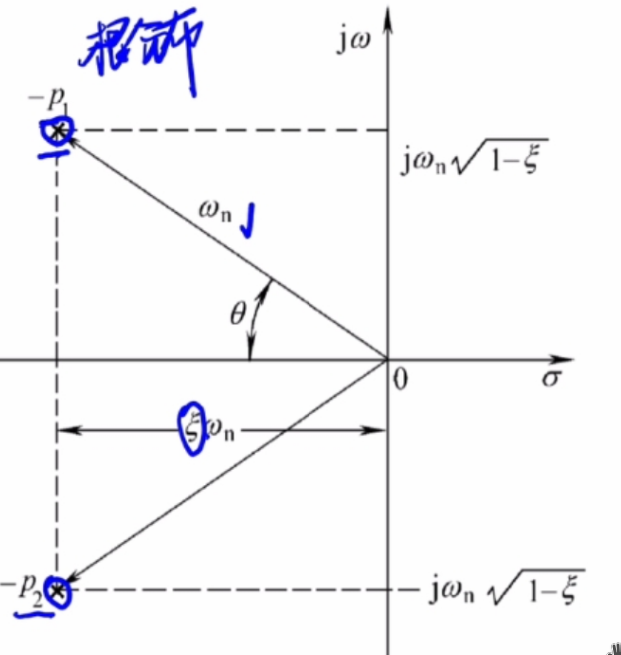
\includegraphics[width=0.4\textwidth]{figures/2021-09-23T004059+0800.png}
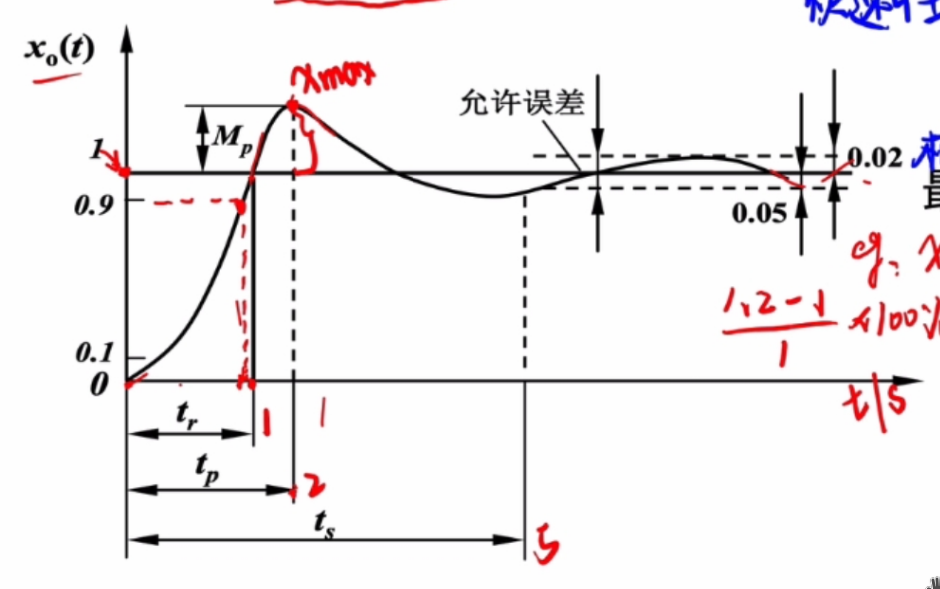
\includegraphics[width=0.5\textwidth]{figures/2021-09-23T004313+0800.png}

上升时间:
\begin{equation*}
	t_r = \frac{\pi - \theta}{ \omega_d } = \frac{\pi - \theta}{ \omega_n \sqrt{1 - \xi^2} }
\end{equation*}
\(\xi\)越大,上升时间越大。
这是显然的。
想象一个在油中的弹簧振子,先被压缩。
摩擦系数越大,达到平衡位置所花时间越长。

峰值(peak)时间:
\begin{equation}
	t_p = \frac{\pi}{ \omega_n \sqrt{1-\xi^2} }
\end{equation}
\(\xi\)越大,peak time 越大
调节时间:
\begin{equation*}
	t_s = \frac{3.5}{\xi \omega_n}
\end{equation*}

\(\xi\)越大,调节时间越小
这是显然的。
想象一个在油中的弹簧振子,先被压缩。
摩擦系数越大,更快静止。

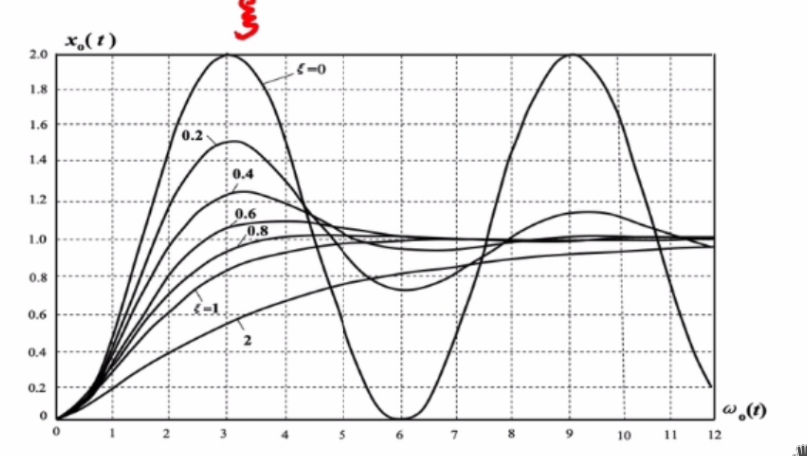
\includegraphics[width=0.5\textwidth]{figures/2021-09-23T011056+0800.png}





%%% vim: set ts=2 sts=2 sw=2 isk+=\: et cc=+1 formatoptions+=mM:
